%% ============================================================
%% Football Possession Intelligence API — Reporte Final
%% Maestría en Ciencia de Datos — Aprendizaje Profundo
%% ============================================================
\documentclass[12pt,a4paper]{article}

%% ── Paquetes ──────────────────────────────────────────────────
\usepackage[utf8]{inputenc}
\usepackage[T1]{fontenc}
\usepackage[spanish]{babel}
\usepackage{lmodern}
\usepackage{geometry}
\geometry{top=2.5cm,bottom=2.5cm,left=3cm,right=2.5cm,headheight=14pt}

\usepackage{amsmath,amssymb}
\usepackage{graphicx}
\usepackage{float}
\usepackage{booktabs}
\usepackage{tabularx}
\usepackage{multirow}
\usepackage{array}
\usepackage{xcolor}
\usepackage{hyperref}
\usepackage{caption}
\usepackage{subcaption}
\usepackage{listings}
\usepackage{enumitem}
\usepackage{fancyhdr}
\usepackage{titlesec}
\usepackage{parskip}
\usepackage{microtype}
\usepackage{tikz}
\usetikzlibrary{shapes.geometric, arrows.meta, positioning, calc}

%% ── Colores ───────────────────────────────────────────────────
\definecolor{primary}{HTML}{1e40af}
\definecolor{accent}{HTML}{dc2626}
\definecolor{neutral}{HTML}{475569}
\definecolor{lightbg}{HTML}{f1f5f9}
\definecolor{codebg}{HTML}{1e293b}
\definecolor{codetext}{HTML}{e2e8f0}

%% ── Hyperref ──────────────────────────────────────────────────
\hypersetup{
    colorlinks=true, linkcolor=primary, citecolor=primary,
    urlcolor=primary, pdftitle={PitchView — Football Possession Intelligence},
    pdfauthor={MCD --- Aprendizaje Profundo}
}

%% ── Código ────────────────────────────────────────────────────
\lstset{
    basicstyle=\ttfamily\footnotesize\color{codetext},
    backgroundcolor=\color{codebg},
    frame=single, rulecolor=\color{neutral},
    breaklines=true, captionpos=b,
    keywordstyle=\color{cyan}\bfseries,
    commentstyle=\color{gray},
    stringstyle=\color{yellow!80!white},
    numbers=left, numberstyle=\tiny\color{gray},
    xleftmargin=1.5em, framexleftmargin=1.5em,
}

%% ── Headers ───────────────────────────────────────────────────
\pagestyle{fancy}
\fancyhf{}
\fancyhead[L]{\small\textcolor{neutral}{PitchView --- Football Possession Intelligence}}
\fancyhead[R]{\small\textcolor{neutral}{\thepage}}
\renewcommand{\headrulewidth}{0.3pt}

%% ── Títulos ───────────────────────────────────────────────────
\titleformat{\section}{\large\bfseries\color{primary}}{}{0em}{}[\titlerule]
\titleformat{\subsection}{\normalsize\bfseries\color{neutral}}{}{0em}{}
\titleformat{\subsubsection}{\normalsize\itshape}{}{0em}{}

%% ── Comandos útiles ───────────────────────────────────────────
\newcommand{\metric}[1]{\textbf{\textcolor{primary}{#1}}}
\newcommand{\model}[1]{\texttt{#1}}
\newcommand{\code}[1]{\texttt{\small #1}}
\newcommand{\placeholder}[1]{%
    \begin{center}
    \colorbox{lightbg}{\parbox{0.85\linewidth}{%
        \centering\vspace{1em}
        \textcolor{neutral}{\large $\square$}\\[0.4em]
        \textcolor{neutral}{\small\textit{#1}}
        \vspace{1em}
    }}
    \end{center}
}

%% ─────────────────────────────────────────────────────────────
\begin{document}

%% ── PORTADA ──────────────────────────────────────────────────
\begin{titlepage}
    \centering
    \vspace*{1.2cm}

    % Línea decorativa superior
    {\color{primary}\rule{\linewidth}{2pt}\par}
    \vspace{0.6cm}

    {\fontsize{32}{38}\selectfont\bfseries\color{primary}
     PitchView\\[0.2em]
     Football Possession\\[0.2em]
     Intelligence API\par}

    \vspace{0.5cm}
    {\color{primary}\rule{\linewidth}{0.8pt}\par}
    \vspace{0.8cm}

    {\large\color{neutral}
     Predicción de la probabilidad de disparo\\[0.2em]
     a partir de secuencias de posesión en fútbol\\[0.2em]
     mediante aprendizaje profundo\par}

    \vspace{1cm}
    {\large\bfseries\color{neutral}
     Luis Alejandro Guillén Alvarez \normalfont\textcolor{neutral}{· 0234598}\\[0.3em]
     \bfseries Enrique Ulises Báez Gómez Tagle \normalfont\textcolor{neutral}{· 0241823}\par}

    \vspace{0.8cm}

    % Tarjetas de métricas clave
    \begin{tikzpicture}
        % Card 1
        \fill[primary!12, rounded corners=6pt] (0,0) rectangle (3.6,1.8);
        \node[align=center] at (1.8,1.1) {\small\color{neutral} PR-AUC (prueba)};
        \node[align=center] at (1.8,0.5) {\Large\bfseries\color{primary} 0.870};
        % Card 2
        \fill[primary!12, rounded corners=6pt] (4,0) rectangle (7.6,1.8);
        \node[align=center] at (5.8,1.1) {\small\color{neutral} Posesiones};
        \node[align=center] at (5.8,0.5) {\Large\bfseries\color{primary} 21{,}080};
        % Card 3
        \fill[primary!12, rounded corners=6pt] (8,0) rectangle (11.6,1.8);
        \node[align=center] at (9.8,1.1) {\small\color{neutral} Partidos analizados};
        \node[align=center] at (9.8,0.5) {\Large\bfseries\color{primary} 127};
        % Card 4
        \fill[primary!12, rounded corners=6pt] (0,-2.2) rectangle (3.6,-0.4);
        \node[align=center] at (1.8,-0.9) {\small\color{neutral} Modelo};
        \node[align=center] at (1.8,-1.6) {\large\bfseries\color{primary} GRU};
        % Card 5
        \fill[primary!12, rounded corners=6pt] (4,-2.2) rectangle (7.6,-0.4);
        \node[align=center] at (5.8,-0.9) {\small\color{neutral} Competencias};
        \node[align=center] at (5.8,-1.6) {\large\bfseries\color{primary} 4 ligas};
        % Card 6
        \fill[primary!12, rounded corners=6pt] (8,-2.2) rectangle (11.6,-0.4);
        \node[align=center] at (9.8,-0.9) {\small\color{neutral} Mejora vs.\ baseline};
        \node[align=center] at (9.8,-1.6) {\large\bfseries\color{primary} +30.7 pp};
    \end{tikzpicture}

    \vfill

    {\large\bfseries Maestría en Ciencia de Datos\par}
    \vspace{0.2cm}
    {\normalsize Curso: Aprendizaje Profundo\par}
    \vspace{0.2cm}
    {\normalsize\color{neutral} Junio 2026\par}
    \vspace{0.2cm}
    {\small Plataforma en vivo: \href{https://srv7050.tailc60ea4.ts.net/}{srv7050.tailc60ea4.ts.net}\par}

\end{titlepage}

%% ── RESUMEN ──────────────────────────────────────────────────
\begin{abstract}
\noindent
Este reporte documenta el desarrollo de un sistema de aprendizaje profundo para
estimar la probabilidad de que una posesión ofensiva en fútbol termine en disparo:
$P(\text{disparo} \mid \text{posesión})$.
El sistema procesa secuencias de eventos de StatsBomb Open Data correspondientes a
127 partidos de cuatro competencias europeas (Bundesliga 2023/24, La Liga 2020/21
y Ligue~1 2021/22 + 2022/23), produciendo un total de 21{,}080 posesiones etiquetadas.

El modelo principal es una red recurrente tipo GRU (Gated Recurrent Unit) de dos capas
que opera sobre secuencias de eventos codificados con 40 características por paso temporal.
Se compara contra un modelo de regresión logística entrenado sobre características
agregadas por posesión.

El GRU alcanza un \metric{PR-AUC de 0.852 en validación} y \metric{0.870 en prueba},
superando al baseline en $+27$ puntos porcentuales. Los resultados se obtienen sin
fuga de datos entre conjuntos (split por \texttt{match\_id}, con estratificación
por competencia) y con exclusión explícita de los eventos de disparo del vector
de entrada para garantizar una tarea de predicción causal.

El sistema es productizado a través de una API REST con FastAPI
(\code{/v1/predict-possession}) y un frontend interactivo en React con visualización
de trayectorias en campo y un medidor de probabilidad.
\end{abstract}

\newpage
\tableofcontents
\newpage

%% ═══════════════════════════════════════════════════════════════
\section{Introducción}

\subsection{El problema de negocio}

El fútbol moderno mueve miles de millones de dólares al año a través de fichajes,
patrocinios, derechos televisivos y apuestas deportivas. En este contexto,
\textbf{entender qué hace peligrosa una jugada} —antes de que ocurra el disparo—
tiene valor directo para múltiples actores del ecosistema:

\begin{itemize}[leftmargin=1.5em]
    \item \textbf{Cuerpos técnicos y analistas tácticos:} identificar qué tipo de
          posesiones genera riesgo real para el rival o para el propio equipo.
          Un entrenador puede revisar en segundos las 10 posesiones más peligrosas
          cedidas en el último partido sin necesidad de ver horas de video.

    \item \textbf{Scouts y departamentos de captación:} evaluar qué tan «amenazante»
          es el juego colectivo de un equipo más allá de estadísticas superficiales
          como porcentaje de posesión o número de remates.

    \item \textbf{Medios y plataformas de \textit{broadcasting}:} enriquecer la
          retransmisión en vivo con una capa de inteligencia que señale jugadas
          de alto peligro antes de que terminen en gol, incrementando el engagement
          de la audiencia.

    \item \textbf{Plataformas de apuestas deportivas:} cuantificar la presión
          ofensiva de un equipo en tiempo real durante el partido como señal
          complementaria para mercados de gol siguiente / corners / disparos.
\end{itemize}

La métrica clave que responde a estas necesidades es:
\[
    P(\text{disparo} \mid \text{posesión})
\]
es decir, la probabilidad de que una posesión ofensiva \emph{termine en intento de
gol}. A diferencia del \textit{Expected Goals} ($xG$), que puntúa la calidad de
un disparo ya ocurrido, esta métrica cuantifica la \emph{peligrosidad de la
construcción} incluso antes de que exista el disparo.

\subsection{Contexto técnico y motivación}

Las métricas tradicionales de fútbol (posesión \%, número de disparos, pases
completados) son estadísticas de resumen que pierden toda la información
\emph{secuencial}: la forma en que una jugada se construye, el orden de las
acciones, cómo progresa el equipo hacia la portería. Un equipo puede tener el 60\%
de la posesión con jugadas inocuas, mientras otro con el 40\% genera el doble de
peligro real.

El modelado de posesiones como secuencias —usando redes neuronales recurrentes—
permite capturar exactamente esa estructura temporal: quién pasó a quién, desde
dónde y hacia dónde, bajo qué presión, durante cuánto tiempo.

\subsection{Objetivo principal}

Construir un sistema end-to-end que, dada la secuencia de eventos de una posesión,
estime en tiempo real la probabilidad de que termine en disparo:

\begin{equation}
    P(\text{disparo} \mid e_1, e_2, \ldots, e_T)
    \label{eq:objetivo}
\end{equation}

donde $e_t$ es el $t$-ésimo evento (pase, conducción, regate, etc.) y $T$ es la
longitud variable de la secuencia. El sistema expone esta predicción a través de
una API REST y una interfaz visual interactiva.

\subsection{Alcance del proyecto}

\begin{itemize}[leftmargin=1.5em]
    \item Fútbol masculino de clubes europeos con datos abiertos disponibles.
    \item Modelado a nivel de posesión — unidad de análisis = una posesión completa.
    \item Clasificación binaria: ¿termina esta posesión en disparo?
    \item Arquitectura GRU como modelo secuencial principal.
    \item API REST + frontend web como capa de producto.
\end{itemize}

Quedan fuera del alcance: visión computacional sobre video, modelos Transformer,
competencias femeninas o internacionales, y clasificación de calidad del disparo ($xG$).

\subsection{Contribuciones}

\begin{enumerate}[leftmargin=1.5em]
    \item Pipeline reproducible de descarga, parseo y etiquetado de posesiones.
    \item Codificación de eventos en vectores de 40 características con gestión de
          secuencias de longitud variable.
    \item Modelo GRU entrenado sin fuga de datos, con split estratificado por competencia.
    \item Comparativa rigurosa contra baseline tabular (regresión logística).
    \item API REST y frontend interactivo con visualización de campo listos para demo.
\end{enumerate}


%% ═══════════════════════════════════════════════════════════════
\section{Dataset}

\subsection{StatsBomb Open Data}

El dataset utilizado es \textbf{StatsBomb Open Data}, disponible públicamente en
\url{https://github.com/statsbomb/open-data}. StatsBomb es una compañía de
analítica deportiva que publica gratuitamente datos de eventos de partidos
seleccionados para uso académico y de investigación.

Cada partido se representa como una lista de eventos JSON ordenados cronológicamente,
donde cada evento describe una acción individual (pase, conducción, disparo, etc.)
con metadatos espaciales y contextuales.

\subsubsection{Campos disponibles por evento}

Los campos relevantes para el modelado de posesiones incluyen:

\begin{table}[H]
\centering
\caption{Campos del esquema de eventos StatsBomb utilizados en este proyecto.}
\begin{tabularx}{\linewidth}{lX}
\toprule
\textbf{Campo} & \textbf{Descripción} \\
\midrule
\code{possession}         & Identificador numérico de la posesión dentro del partido \\
\code{type}               & Tipo de evento: \textit{Pass, Carry, Dribble, Shot,} etc. \\
\code{play\_pattern}      & Patrón de inicio: \textit{Regular Play, From Corner,} etc. \\
\code{location}           & Coordenadas $(x, y)$ en campo de $120 \times 80$ metros \\
\code{pass\_end\_location}& Coordenadas de destino del pase \\
\code{carry\_end\_location}& Coordenadas de destino de la conducción \\
\code{duration}           & Duración del evento en segundos \\
\code{under\_pressure}    & Indicador booleano de presión defensiva \\
\code{minute}, \code{second} & Marca temporal en el partido \\
\bottomrule
\end{tabularx}
\label{tab:event_fields}
\end{table}

\subsection{Competencias seleccionadas}

Se seleccionaron cuatro competencias de clubes europeos masculinos con datos de eventos
disponibles. La selección prioriza homogeneidad táctica (exclusión de torneos
internacionales) y volumen de partidos.

\begin{table}[H]
\centering
\caption{Competencias incluidas en el dataset de entrenamiento.}
\begin{tabular}{llccc}
\toprule
\textbf{Competencia} & \textbf{Temporada} & \textbf{ID comp.} & \textbf{ID temp.} & \textbf{Partidos} \\
\midrule
1. Bundesliga & 2023/2024 & 9  & 281 & 34 \\
La Liga       & 2020/2021 & 11 & 90  & 35 \\
Ligue 1       & 2021/2022 & 7  & 108 & 26 \\
Ligue 1       & 2022/2023 & 7  & 235 & 32 \\
\midrule
\multicolumn{4}{r}{\textbf{Total}} & \textbf{127} \\
\bottomrule
\end{tabular}
\label{tab:competitions}
\end{table}

\subsection{Estadísticas del dataset}

A partir de los 127 partidos se extrajeron 21{,}080 posesiones únicas. La distribución
de clases refleja la naturaleza del fútbol: la mayoría de las posesiones no terminan
en disparo.

\begin{table}[H]
\centering
\caption{Estadísticas generales del dataset de posesiones.}
\begin{tabular}{lr}
\toprule
\textbf{Métrica} & \textbf{Valor} \\
\midrule
Total de posesiones      & 21{,}080 \\
Posesiones con disparo   & 3{,}024 (14.3\%) \\
Posesiones sin disparo   & 18{,}056 (85.7\%) \\
Razón de desequilibrio   & $\approx 6:1$ \\
Partidos                 & 127 \\
Promedio posesiones/partido & $\approx 166$ \\
\bottomrule
\end{tabular}
\label{tab:dataset_stats}
\end{table}


%% ═══════════════════════════════════════════════════════════════
\section{Análisis Exploratorio de Datos (EDA)}

\subsection{Distribución de clases}

La figura~\ref{fig:label_dist} muestra la distribución de posesiones con y sin
disparo. El desequilibrio de clases ($\approx 6:1$) es manejable para clasificación
binaria estándar y fue tratado mediante pérdida BCE ponderada durante el entrenamiento
del GRU (peso positivo = $18{,}056 / 3{,}024 \approx 5.97$).

\begin{figure}[H]
    \centering
    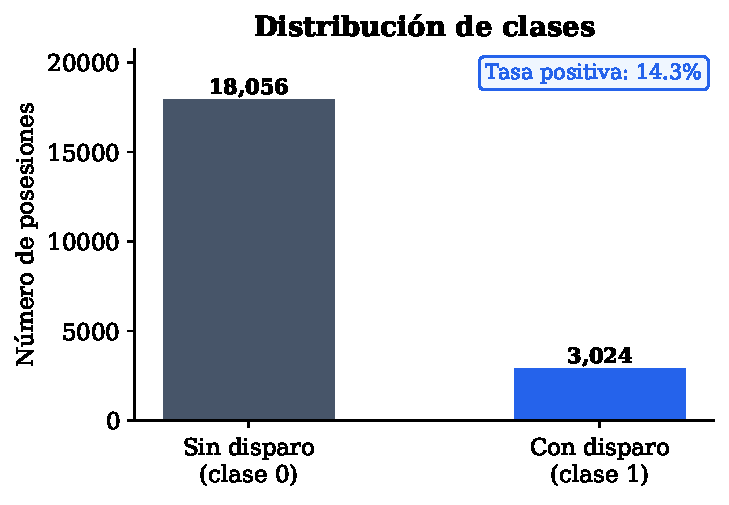
\includegraphics[width=0.55\textwidth]{figures/label_distribution.pdf}
    \caption{Distribución de clases en el dataset completo (21{,}080 posesiones).}
    \label{fig:label_dist}
\end{figure}

\subsection{Tasa de disparo por competencia}

\begin{figure}[H]
    \centering
    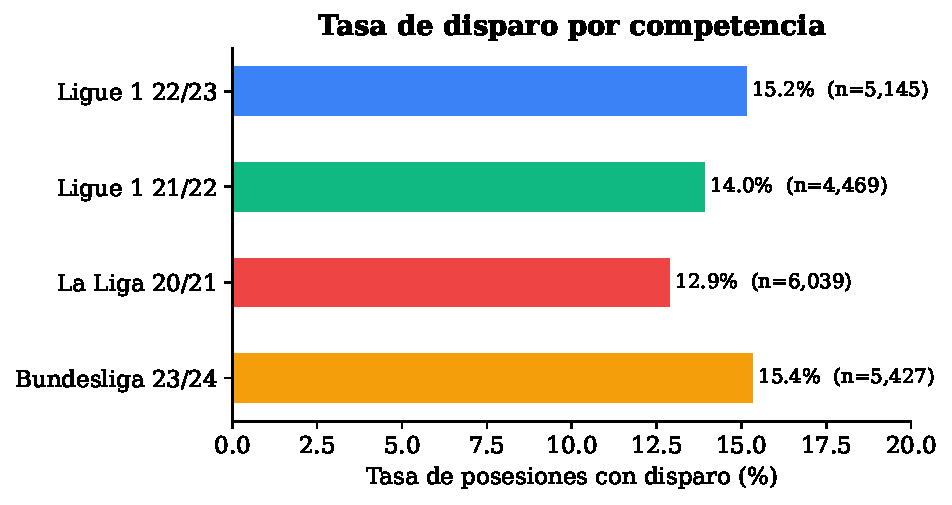
\includegraphics[width=0.78\textwidth]{figures/shot_rate_by_competition.pdf}
    \caption{Porcentaje de posesiones que terminan en disparo por competencia.}
    \label{fig:shot_rate_comp}
\end{figure}

Las cuatro ligas presentan tasas de disparo similares (entre 13\% y 16\%),
lo que indica que el modelo no debería desarrollar sesgos fuertes por competencia
derivados de esta variable.

\subsection{Longitud de secuencia}

\begin{figure}[H]
    \centering
    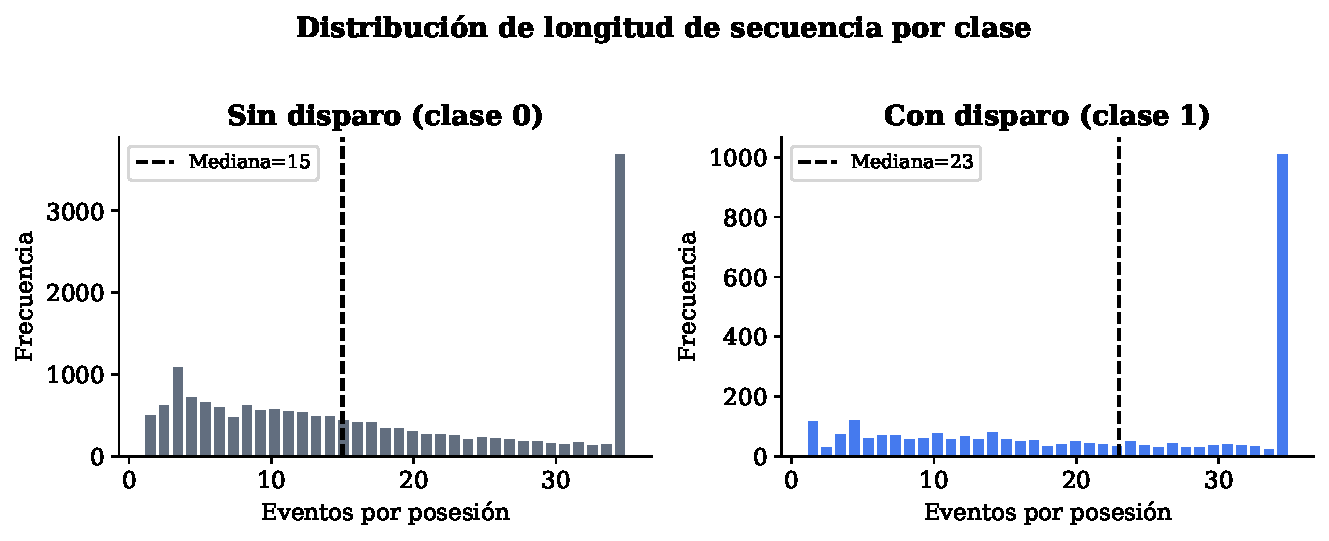
\includegraphics[width=\textwidth]{figures/sequence_length.pdf}
    \caption{Distribución del número de eventos por posesión, separada por clase.
             Las posesiones con disparo tienden a ser más largas.}
    \label{fig:seq_length}
\end{figure}

Las posesiones que terminan en disparo son notoriamente más largas que las que no:
la diferencia en mediana refleja que los equipos construyen jugadas más elaboradas
antes de llegar al disparo. Esta señal es aprovechable por un modelo secuencial.

\subsection{Progresión territorial}

\begin{figure}[H]
    \centering
    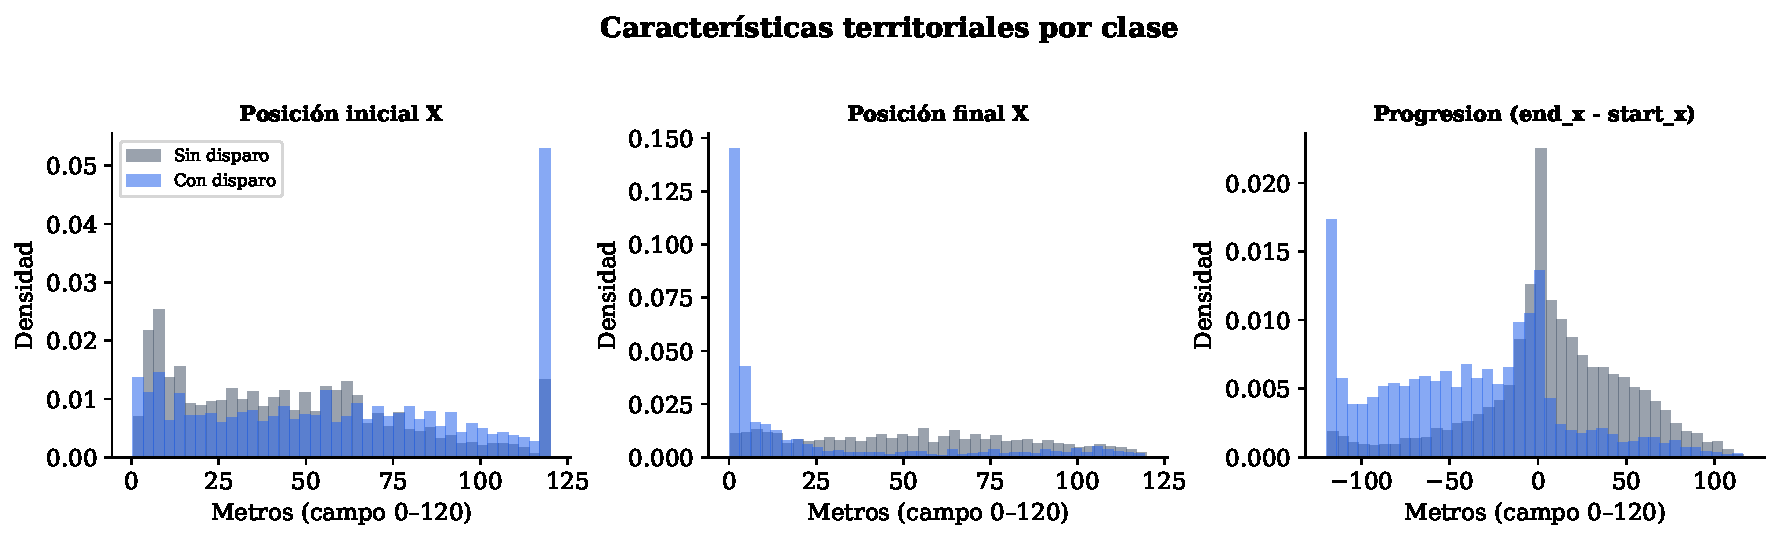
\includegraphics[width=\textwidth]{figures/territory_features.pdf}
    \caption{Distribución de características territoriales: posición inicial,
             posición final y progresión neta. Las posesiones con disparo muestran
             inicio y final más avanzados hacia la portería rival ($x = 120$).}
    \label{fig:territory}
\end{figure}

La posición inicial y final de las posesiones con disparo están significativamente
más adelantadas en el campo. La progresión neta también es mayor, aunque con mayor
varianza (algunas posesiones progresan mucho desde zonas defensivas).

\subsection{Análisis por patrón de juego}

\begin{figure}[H]
    \centering
    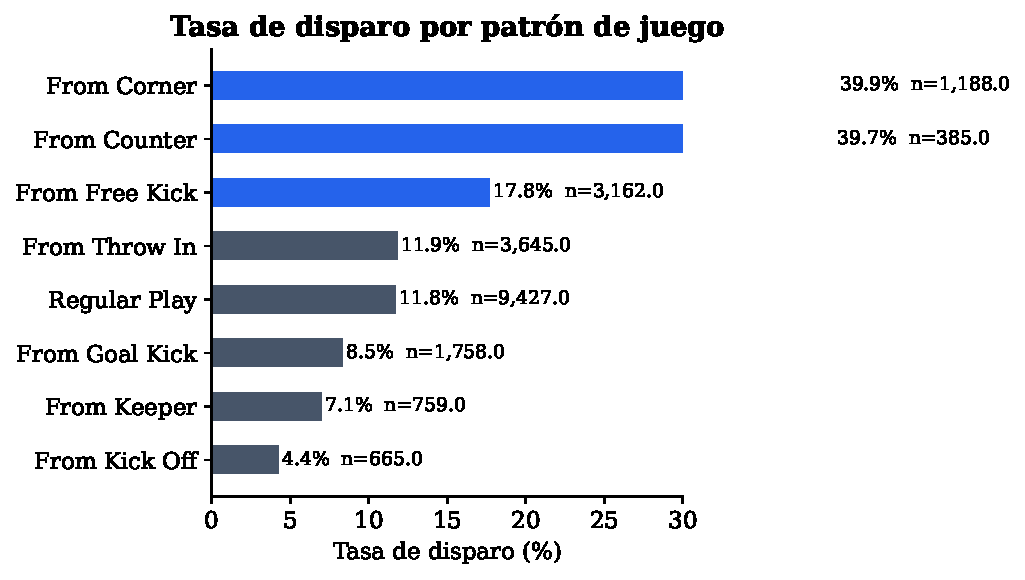
\includegraphics[width=0.88\textwidth]{figures/play_pattern.pdf}
    \caption{Tasa de disparo según el patrón de inicio de posesión.
             El tiro libre y el saque de esquina tienen tasas notablemente mayores.}
    \label{fig:play_pattern}
\end{figure}

Las jugadas a balón parado (tiro libre, saque de esquina) presentan las tasas de
disparo más altas, lo que es coherente con el diseño táctica en fútbol moderno
donde las jugadas ensayadas de este tipo frecuentemente finalizan en remate.


%% ═══════════════════════════════════════════════════════════════
\section{Metodología}

\subsection{Definición formal del problema}

Sea $P_i = (e_1^{(i)}, e_2^{(i)}, \ldots, e_{T_i}^{(i)})$ la secuencia de eventos
de la $i$-ésima posesión, donde cada evento $e_t$ es un vector de características
$\mathbf{x}_t \in \mathbb{R}^{40}$. La etiqueta es:

\begin{equation}
    y_i = \mathbb{1}[\text{la posesión } i \text{ contiene algún evento de tipo \textit{Shot}}]
\end{equation}

El objetivo es aprender una función $f_\theta: \mathbb{R}^{T \times 40} \to [0,1]$ tal que:

\begin{equation}
    \hat{y}_i = f_\theta(\mathbf{x}_1^{(i)}, \ldots, \mathbf{x}_{T_i}^{(i)})
    \approx P(\text{disparo} \mid P_i)
\end{equation}

\textbf{Nota crítica sobre fuga de datos:} Los eventos de tipo \textit{Shot} fueron
\emph{excluidos explícitamente} del vector de entrada. Incluirlos permitiría al modelo
detectar trivialmente la presencia del disparo en la secuencia, invalidando la tarea
de predicción. El modelo ve únicamente los eventos \emph{previos} al disparo (o todos
los eventos en posesiones sin disparo).

\subsection{Pipeline de datos}

El pipeline de procesamiento sigue los siguientes pasos:

\begin{enumerate}[leftmargin=1.5em]
    \item \textbf{Descarga:} Se obtienen los archivos JSON de eventos para los 127
          partidos seleccionados usando la librería \code{statsbombpy}.
    \item \textbf{Agrupación por posesión:} Los eventos se agrupan por el campo
          \code{possession}, que es el identificador asignado por StatsBomb a cada
          posesión dentro de un partido.
    \item \textbf{Filtrado:} Se eliminan eventos de tipo administrativo
          (\textit{Starting XI, Half Start/End, Substitution, Tactical Shift, etc.}).
    \item \textbf{Etiquetado:} Si algún evento de la posesión es de tipo \textit{Shot},
          la posesión recibe etiqueta $y = 1$.
    \item \textbf{Codificación:} Cada evento se codifica en un vector de 40 dimensiones
          (descrito en la sección \ref{sec:features}).
    \item \textbf{Serialización:} Los datos procesados se guardan en formato Parquet
          para reproducibilidad.
\end{enumerate}

\subsection{Ingeniería de características}
\label{sec:features}

Cada evento es representado por un vector $\mathbf{x}_t \in \mathbb{R}^{40}$
compuesto de tres bloques:

\begin{table}[H]
\centering
\caption{Composición del vector de características por evento.}
\begin{tabularx}{\linewidth}{lcX}
\toprule
\textbf{Bloque} & \textbf{Dims} & \textbf{Descripción} \\
\midrule
Tipo de evento (one-hot)    & 23 & Pass, Carry, Dribble, Ball Receipt*, etc. \\
Patrón de juego (one-hot)   & 8  & Regular Play, From Corner, From Free Kick, etc. \\
Zona del campo (one-hot)    & 4  & Defensiva ($x<40$), Media, Atacante ($x>80$), Desconocida \\
\midrule
Características continuas   & 5  & $x_\text{norm}, y_\text{norm}, x_\text{end\_norm}, y_\text{end\_norm}, \text{duration\_norm}$ + \code{under\_pressure} (binario) \\
\midrule
\textbf{Total}              & \textbf{40} & \\
\bottomrule
\end{tabularx}
\label{tab:features}
\end{table}

Las coordenadas se normalizan dividiendo por las dimensiones del campo ($120 \times 80$~m).
La duración se normaliza con un máximo de 10~s. Las secuencias se truncan o rellenan
(\textit{padding}) hasta una longitud máxima de $T_{\max} = 50$ eventos.

\subsection{División de datos}

El dataset se divide a nivel de partido (\texttt{match\_id}), garantizando que
todas las posesiones de un mismo partido pertenezcan al mismo conjunto.
La estratificación por competencia asegura representación de las cuatro ligas
en cada split.

\begin{table}[H]
\centering
\caption{Distribución de partidos y posesiones por split.}
\begin{tabular}{lccccc}
\toprule
\textbf{Split} & \textbf{Ratio} & \textbf{Partidos} & \textbf{Posesiones} & \textbf{Disparos} & \textbf{Tasa} \\
\midrule
Entrenamiento  & 70\% & 88 & 14{,}582 & 2{,}114 & 14.5\% \\
Validación     & 15\% & 19 &  3{,}192 &   457   & 14.3\% \\
Prueba         & 15\% & 20 &  3{,}306 &   453   & 13.7\% \\
\midrule
\textbf{Total} &      & \textbf{127} & \textbf{21{,}080} & \textbf{3{,}024} & \textbf{14.3\%} \\
\bottomrule
\end{tabular}
\label{tab:splits}
\end{table}

\textbf{Reglas de split:}
\begin{itemize}[leftmargin=1.5em, noitemsep]
    \item División por \texttt{match\_id} — ninguna posesión cruza entre splits.
    \item Estratificación por \code{competition\_label} — cada split contiene
          representación de las cuatro competencias.
    \item Semilla fija (\code{random\_state=42}) para reproducibilidad.
\end{itemize}

\subsection{Modelo baseline}

El baseline es una \textbf{regresión logística} entrenada sobre características
\emph{agregadas} a nivel de posesión (sin información secuencial). El preprocesamiento
incluye normalización estándar para variables numéricas y codificación one-hot para
variables categóricas.

\begin{table}[H]
\centering
\caption{Características del modelo baseline (regresión logística).}
\begin{tabularx}{\linewidth}{lX}
\toprule
\textbf{Tipo} & \textbf{Características} \\
\midrule
Numéricas (11) & n\_eventos, n\_pases, n\_conducciones, n\_regates, n\_presiones,
                 n\_acciones\_tercio\_atacante, start\_x, end\_x,
                 progresión, duración\_total, minuto\_inicio \\
Categóricas (3) & zona\_inicio, zona\_final, patrón\_de\_juego \\
\bottomrule
\end{tabularx}
\end{table}

\subsection{Arquitectura GRU}

El modelo principal es una \textbf{GRU (Gated Recurrent Unit)} de dos capas.
La elección de GRU sobre LSTM se justifica por su eficiencia computacional comparable
con rendimiento similar en secuencias de longitud moderada. Se descartó Transformer
en esta versión dado el tamaño del dataset (insuficiente para aprender atención
multi-cabeza de manera estable sin preentrenamiento).

\begin{figure}[H]
\centering
\begin{tikzpicture}[
    box/.style={draw, rounded corners=4pt, fill=primary!10,
                minimum width=4cm, minimum height=0.75cm,
                align=center, font=\small},
    arrow/.style={-{Stealth}, thick, color=primary},
    node distance=0.55cm,
]
    \node[box, fill=neutral!10] (input) {Secuencia de eventos \\ $(B,\,T,\,40)$};
    \node[box, below=of input] (proj)  {Linear $(40 \to 64)$};
    \node[box, below=of proj]  (gru1)  {GRU Capa 1 \quad $(64 \to 128)$ \\ dropout $= 0.3$};
    \node[box, below=of gru1]  (gru2)  {GRU Capa 2 \quad $(128 \to 128)$ \\ dropout $= 0.3$};
    \node[box, below=of gru2, fill=accent!10] (hn) {$h_n[-1]$ — último estado \\ $(B,\,128)$};
    \node[box, below=of hn]    (drop)  {Dropout $(p=0.3)$};
    \node[box, below=of drop]  (head)  {Linear $(128 \to 1)$ + Sigmoid};
    \node[box, below=of head, fill=primary!20] (out)
        {$\hat{y} = P(\text{disparo} \mid \text{posesión})$};

    \foreach \a/\b in {input/proj, proj/gru1, gru1/gru2, gru2/hn, hn/drop, drop/head, head/out}
        \draw[arrow] (\a) -- (\b);
\end{tikzpicture}
\caption{Arquitectura del modelo GRU para predicción de disparo en posesión.}
\label{fig:gru_arch}
\end{figure}

\begin{table}[H]
\centering
\caption{Hiperparámetros del modelo GRU.}
\begin{tabular}{lc}
\toprule
\textbf{Hiperparámetro} & \textbf{Valor} \\
\midrule
Tamaño de entrada        & 40 \\
Proyección               & 64 \\
Celdas ocultas           & 128 \\
Capas GRU                & 2 \\
Dropout                  & 0.3 \\
Parámetros totales       & 176{,}385 \\
\midrule
Función de pérdida       & BCE ponderada ($w_+ \approx 5.97$) \\
Optimizador              & AdamW ($\alpha = 3\times10^{-4}$, $\lambda = 10^{-4}$) \\
Scheduler                & CosineAnnealingLR \\
Épocas máximas           & 40 \\
Paciencia (early stop)   & 8 épocas (por PR-AUC en validación) \\
Tamaño de batch          & 256 \\
Longitud máx. secuencia  & 50 \\
\bottomrule
\end{tabular}
\label{tab:hyperparams}
\end{table}

\textbf{Gestión de longitud variable:} Se usa \code{pack\_padded\_sequence} de PyTorch
para evitar que el padding influya en la actualización de los estados ocultos.
El estado final $h_n[-1]$ (última capa, último paso temporal real) se usa como
representación de la posesión completa.

\textbf{Entorno de entrenamiento:} GPU NVIDIA GeForce RTX 5080 (16~GB VRAM),
PyTorch 2.10.0 con soporte CUDA 13.0.


%% ═══════════════════════════════════════════════════════════════
\section{Resultados}

\subsection{Curvas de entrenamiento}

\begin{figure}[H]
    \centering
    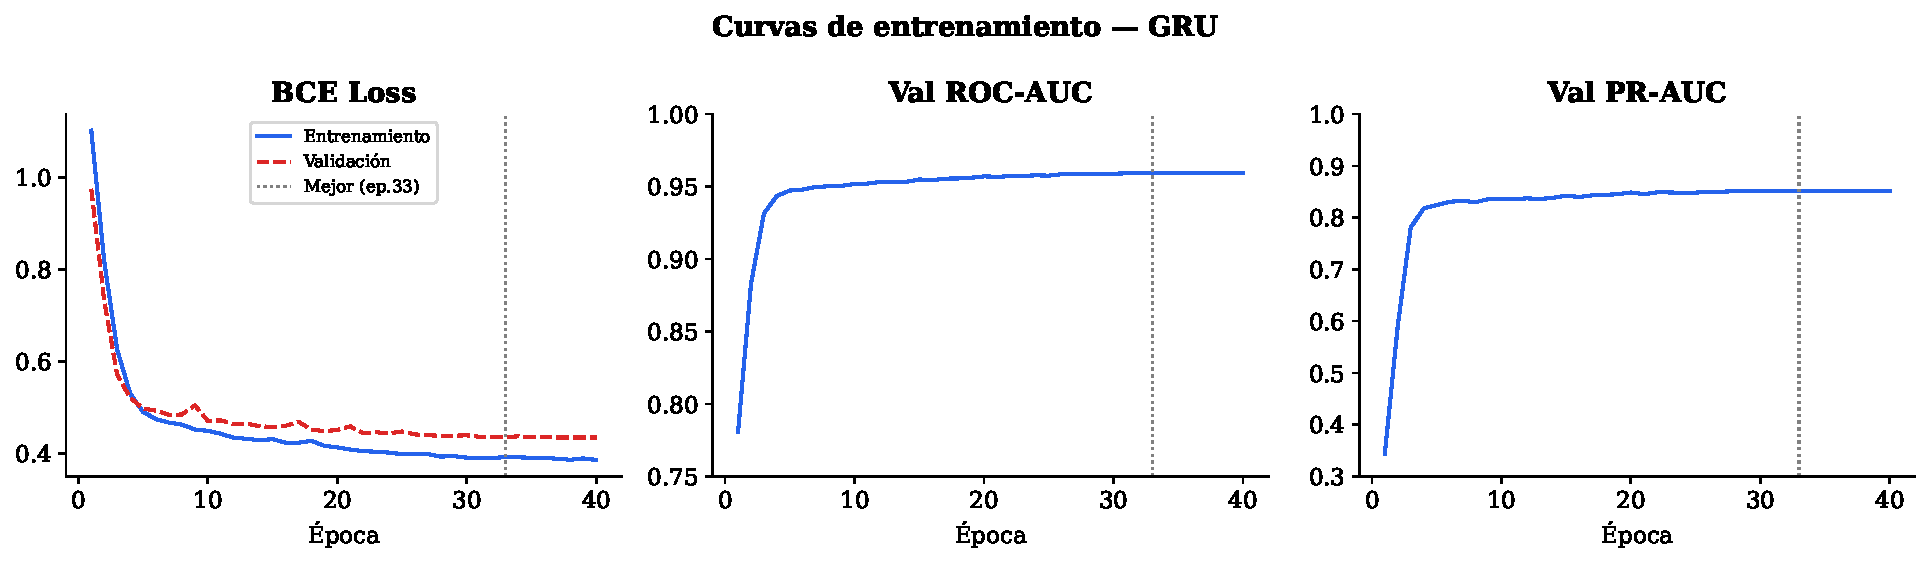
\includegraphics[width=\textwidth]{figures/training_curves.pdf}
    \caption{Evolución de la pérdida BCE, ROC-AUC y PR-AUC en validación durante
             el entrenamiento. La línea punteada vertical indica la época del mejor
             checkpoint (seleccionado por PR-AUC en validación).}
    \label{fig:training_curves}
\end{figure}

El modelo converge establemente a lo largo de las 40 épocas. La pérdida de validación
no diverge respecto a la de entrenamiento, indicando ausencia de sobreajuste severo.
El PR-AUC en validación alcanza un plateau a partir de la época~20 en torno a $0.85$.

\subsection{Métricas de evaluación}

\begin{figure}[H]
    \centering
    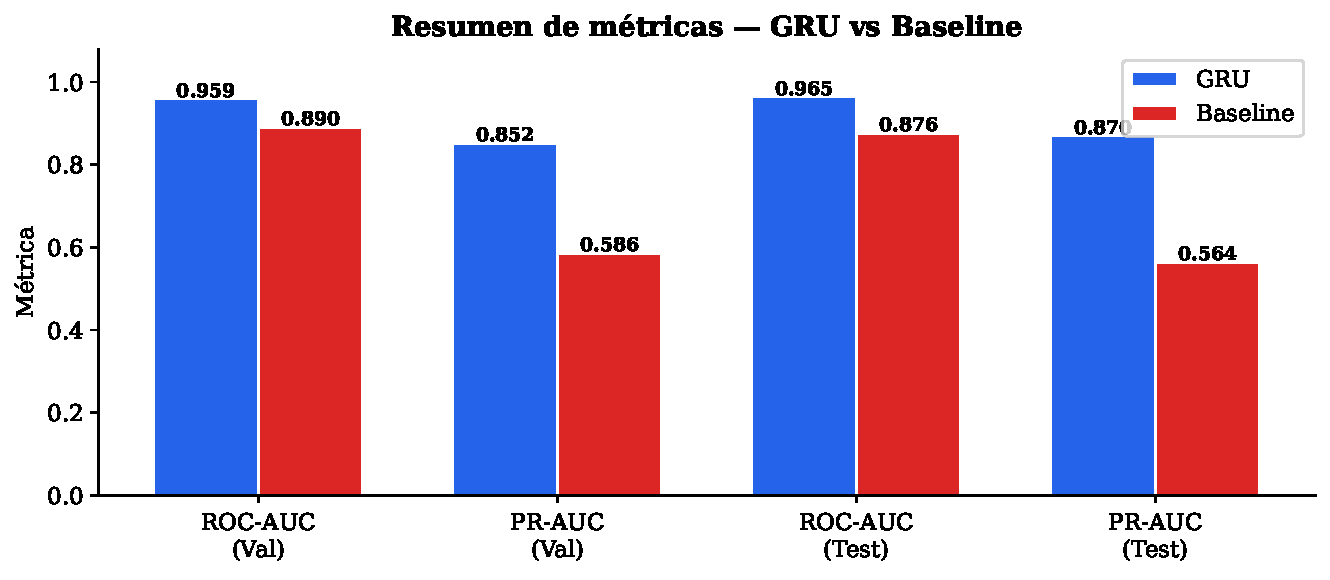
\includegraphics[width=0.88\textwidth]{figures/metrics_summary.pdf}
    \caption{Comparativa de métricas principales entre GRU y baseline de regresión
             logística, en validación y prueba.}
    \label{fig:metrics_summary}
\end{figure}

\begin{table}[H]
\centering
\caption{Resultados completos de evaluación — GRU vs. Baseline.}
\begin{tabular}{llcccc}
\toprule
\textbf{Modelo} & \textbf{Split} & \textbf{ROC-AUC} & \textbf{PR-AUC}
                 & \textbf{Log-Loss} & \textbf{Brier} \\
\midrule
\multirow{2}{*}{GRU}
    & Validación & \metric{0.9592} & \metric{0.8522} & 0.2515 & 0.0759 \\
    & Prueba     & \metric{0.9649} & \metric{0.8703} & 0.2310 & 0.0702 \\
\midrule
\multirow{2}{*}{Baseline (LR)}
    & Validación & 0.8904 & 0.5857 & 0.4515 & 0.1438 \\
    & Prueba     & 0.8756 & 0.5635 & 0.4451 & 0.1409 \\
\midrule
\multicolumn{2}{l}{\textit{Mejora GRU vs Baseline (Test PR-AUC)}}
    & \multicolumn{4}{c}{\textbf{+30.7 pp}} \\
\bottomrule
\end{tabular}
\label{tab:results_main}
\end{table}

El PR-AUC es la métrica principal por ser más informativa que el ROC-AUC en
presencia de desequilibrio de clases. Un modelo aleatorio obtendría PR-AUC $\approx 0.143$
(igual a la tasa base); el GRU alcanza $0.870$ en prueba, superando al baseline en
más del doble.

\subsection{Curvas ROC y Precisión-Recall}

\begin{figure}[H]
    \centering
    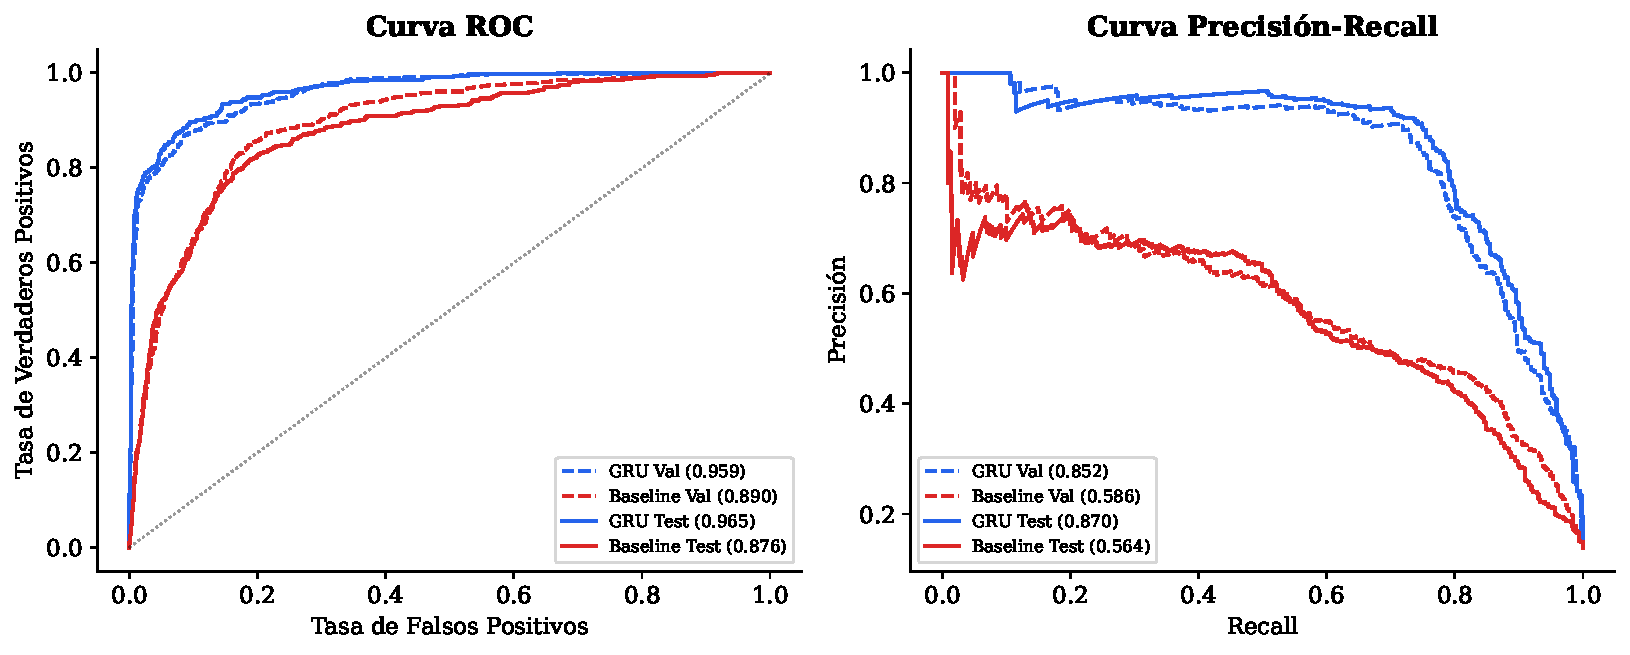
\includegraphics[width=\textwidth]{figures/roc_pr_curves.pdf}
    \caption{Curvas ROC (izquierda) y Precisión-Recall (derecha) para GRU y baseline,
             en validación (línea discontinua) y prueba (línea sólida).}
    \label{fig:roc_pr}
\end{figure}

Las curvas muestran que el GRU domina al baseline en ambas métricas y en ambos
conjuntos. La consistencia entre validación y prueba confirma buena generalización.

\subsection{Resultados por competencia}

\begin{figure}[H]
    \centering
    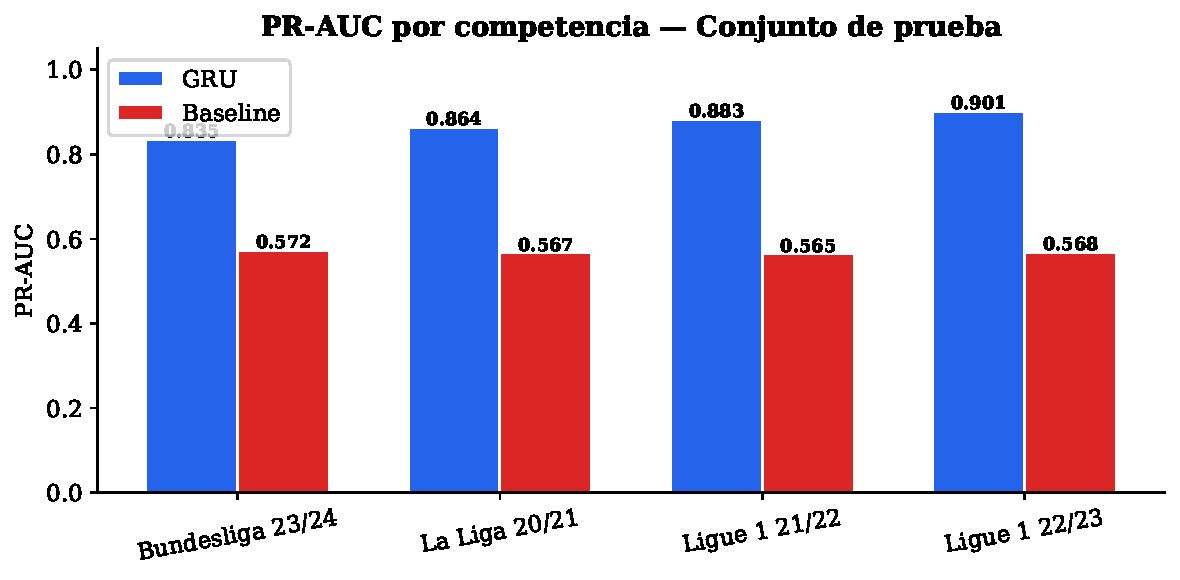
\includegraphics[width=0.88\textwidth]{figures/per_competition_pr_auc.pdf}
    \caption{PR-AUC por competencia en el conjunto de prueba. El GRU supera al
             baseline en todas las ligas sin excepción.}
    \label{fig:per_comp}
\end{figure}

\begin{table}[H]
\centering
\caption{Resultados por competencia en el conjunto de prueba.}
\begin{tabular}{lcccc}
\toprule
\textbf{Competencia} & \multicolumn{2}{c}{\textbf{GRU}} & \multicolumn{2}{c}{\textbf{Baseline}} \\
\cmidrule(lr){2-3}\cmidrule(lr){4-5}
 & ROC-AUC & PR-AUC & ROC-AUC & PR-AUC \\
\midrule
Bundesliga 2023/24 & 0.9564 & 0.8350 & 0.8840 & 0.5723 \\
La Liga 2020/21    & 0.9652 & 0.8643 & 0.8861 & 0.5672 \\
Ligue 1 2021/22    & 0.9643 & 0.8828 & 0.8639 & 0.5651 \\
Ligue 1 2022/23    & 0.9728 & 0.9013 & 0.8684 & 0.5680 \\
\midrule
\textbf{Total}     & \textbf{0.9649} & \textbf{0.8703} & \textbf{0.8756} & \textbf{0.5635} \\
\bottomrule
\end{tabular}
\label{tab:per_comp}
\end{table}

El modelo generaliza de forma consistente entre ligas, con PR-AUC entre 0.835 y 0.901.
La Ligue 1 2022/23 presenta el mejor desempeño, posiblemente relacionado con el mayor
volumen de posesiones disponibles en ese conjunto de prueba.

\subsection{Calibración}

\begin{figure}[H]
    \centering
    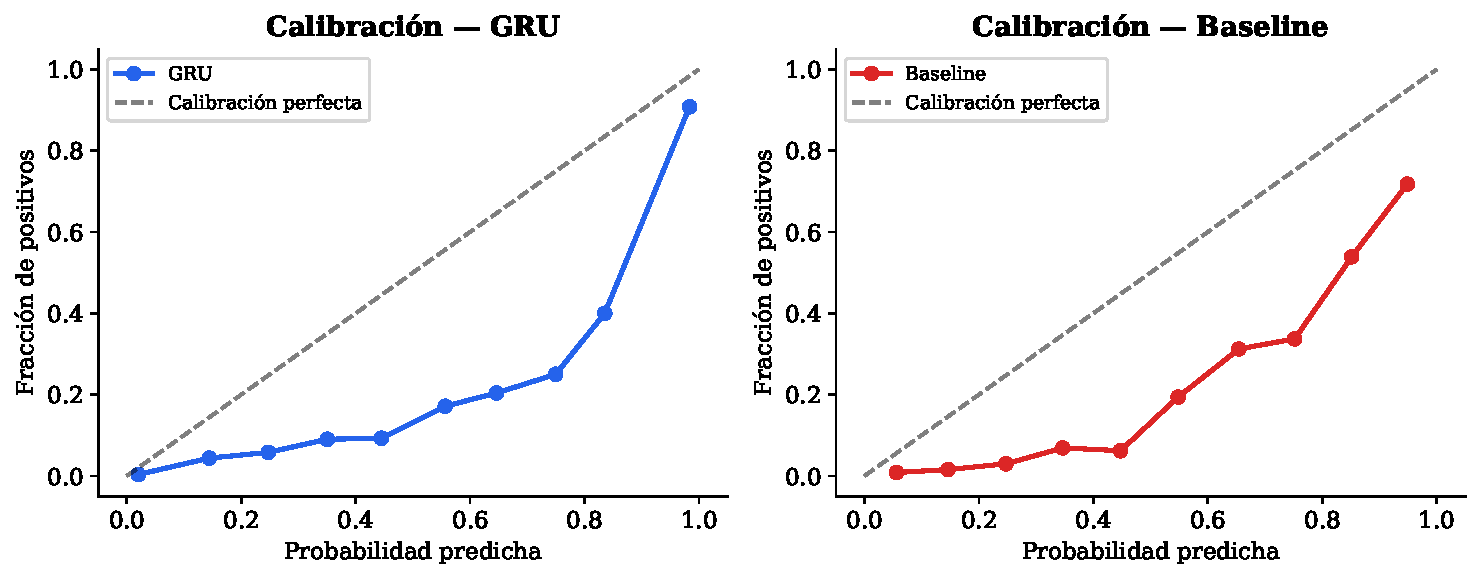
\includegraphics[width=\textwidth]{figures/calibration_curves.pdf}
    \caption{Curvas de calibración para GRU (izquierda) y baseline (derecha)
             en el conjunto de validación. El eje diagonal representa calibración perfecta.}
    \label{fig:calibration}
\end{figure}

El GRU muestra mejor calibración que el baseline: sus probabilidades predichas se
aproximan más a la calibración perfecta (diagonal), aunque con ligera sobreconfianza
en el rango $[0.3, 0.7]$. El baseline sobreestima sistemáticamente en todos los
rangos. Una isotonic regression o Platt scaling podría mejorar la calibración del
GRU en producción.


%% ═══════════════════════════════════════════════════════════════
\section{API y Aplicación Web}

\subsection{Visión general del producto}

El sistema va más allá del modelo estadístico: el objetivo es que cualquier analista,
periodista o desarrollador pueda \textbf{consumir las predicciones sin necesidad de
conocimiento técnico en ML}. Para ello, el modelo entrenado se empaqueta en dos capas:

\begin{enumerate}[leftmargin=1.5em, noitemsep]
    \item \textbf{API REST} — interfaz programática que acepta eventos de posesión en
          JSON y devuelve la probabilidad de disparo. Consumible desde cualquier lenguaje
          o plataforma.
    \item \textbf{Frontend web} — aplicación React con visualización interactiva
          del campo, medidor de peligrosidad y línea de tiempo de eventos.
\end{enumerate}

\subsection{Arquitectura técnica del sistema}

\begin{figure}[H]
\centering
\begin{tikzpicture}[
    comp/.style={draw, rounded corners=6pt, minimum width=3.5cm,
                 minimum height=1.3cm, font=\small, align=center},
    arrow/.style={-{Stealth}, thick},
    node distance=1.8cm,
]
    \node[comp, fill=primary!15] (fe)    {Frontend\\React + Vite\\puerto 5173};
    \node[comp, fill=accent!10, right=2.2cm of fe]    (be)    {Backend\\FastAPI\\puerto 8000};
    \node[comp, fill=neutral!15, right=2.2cm of be]   (model) {Modelos\\GRU + Baseline\\\texttt{.pt} / \texttt{.pkl}};

    \draw[arrow] (fe.east) -- node[above, font=\footnotesize]{\texttt{POST /v1/predict}} (be.west);
    \draw[arrow] (be.west) -- ++(0,-0.6) -| (fe.south);
    \draw[arrow, dashed] (be.east) -- node[above, font=\footnotesize]{carga lazy} (model.west);
\end{tikzpicture}
\caption{Componentes del sistema. El frontend consume la API REST; los modelos se
         cargan en memoria al primer request (\textit{lazy loading}).}
\label{fig:arch_system}
\end{figure}

\textbf{Stack tecnológico:}
\begin{itemize}[leftmargin=1.5em, noitemsep]
    \item \textbf{Backend:} Python 3.12, FastAPI, Uvicorn, PyTorch, scikit-learn.
          CORS habilitado para comunicación con el frontend local.
          Documentación automática disponible en \code{/docs} (Swagger UI).
    \item \textbf{Frontend:} React 18, TypeScript, Vite, Tailwind CSS.
          Visualización de campo con SVG nativo (escala $120 \times 80$ m
          $\to 600 \times 400$ px). Sin dependencias de mapas externos.
\end{itemize}

\subsection{Endpoints de la API}

\begin{table}[H]
\centering
\caption{Endpoints expuestos por el backend FastAPI.}
\begin{tabularx}{\linewidth}{llX}
\toprule
\textbf{Método} & \textbf{Ruta} & \textbf{Descripción} \\
\midrule
GET  & \code{/health}                & Estado del servicio y modelos cargados \\
GET  & \code{/v1/models}             & Lista de modelos disponibles con metadatos \\
POST & \code{/v1/predict-possession} & Probabilidad de disparo para una posesión \\
POST & \code{/v1/analyze-match}      & Rankeo de todas las posesiones de un partido \\
\bottomrule
\end{tabularx}
\end{table}

\subsubsection{Predicción de una posesión (\texttt{/v1/predict-possession})}

El endpoint principal acepta una lista de eventos en formato JSON y retorna la
probabilidad predicha. Se puede especificar qué modelo usar: \code{"gru"} o
\code{"baseline"}.

\begin{lstlisting}[language=Python, caption={Request de predicción — ataque en campo rival bajo presión.}]
POST /v1/predict-possession
{
  "model": "gru",
  "events": [
    {"event_type": "Pass",    "play_pattern": "Regular Play",
     "x": 75.0, "y": 40.0,  "end_x": 88.0, "end_y": 35.0,
     "duration": 0.8,        "under_pressure": 0},
    {"event_type": "Carry",  "play_pattern": "Regular Play",
     "x": 88.0, "y": 35.0,  "end_x": 105.0, "end_y": 38.0,
     "duration": 1.4,        "under_pressure": 1},
    {"event_type": "Dribble","play_pattern": "Regular Play",
     "x": 105.0,"y": 38.0,  "end_x": null,  "end_y": null,
     "duration": 0.5,        "under_pressure": 1}
  ]
}
\end{lstlisting}

\begin{lstlisting}[language=Python, caption={Respuesta — probabilidad de disparo y metadatos.}]
{
  "shot_probability": 0.6821,
  "model_used": "gru",
  "n_events": 3,
  "model_version": "1.0.0",
  "timestamp": "2026-06-23T17:45:12+00:00"
}
\end{lstlisting}

Un valor de $0.68$ indica que posesiones con este patrón terminan en disparo en
$\approx 68\%$ de los casos según lo aprendido por el modelo.

\subsubsection{Análisis completo de partido (\texttt{/v1/analyze-match})}

Este endpoint recibe todas las posesiones de un partido y devuelve un ranking
ordenado de mayor a menor peligrosidad. Útil para generar resúmenes post-partido
automáticos sin revisión manual de video.

\begin{lstlisting}[language=Python, caption={Respuesta de analyze-match (extracto).}]
{
  "possessions_ranked": [
    {"possession_id": 47, "shot_probability": 0.891, "n_events": 12,
     "zone": "attacking", "play_pattern": "From Corner"},
    {"possession_id": 83, "shot_probability": 0.834, "n_events": 8,
     "zone": "attacking", "play_pattern": "Regular Play"},
    ...
  ],
  "match_summary": {
    "total_possessions": 162,
    "high_danger": 18,
    "medium_danger": 41,
    "low_danger": 103
  }
}
\end{lstlisting}

\subsection{Frontend interactivo}

\subsubsection{Flujo de uso}

El frontend está diseñado para ser usado por analistas sin conocimientos de
programación. El flujo típico es:

\begin{enumerate}[leftmargin=1.5em]
    \item \textbf{Seleccionar escenario:} el usuario elige uno de los tres escenarios
          de posesión predefinidos (o puede enviar su propia secuencia de eventos
          vía la API directamente).
    \item \textbf{Elegir modelo:} selecciona entre el GRU (mayor precisión) y el
          baseline de regresión logística (más interpretable, sin GPU).
    \item \textbf{Enviar a la API:} con un clic, el frontend hace un \texttt{POST}
          al backend y recibe la probabilidad en milisegundos.
    \item \textbf{Interpretar:} el resultado se muestra en tres componentes visuales
          simultáneos: campo, gauge y línea de tiempo.
\end{enumerate}

\subsubsection{Escenarios predefinidos}

\begin{table}[H]
\centering
\caption{Escenarios de posesión predefinidos en el frontend.}
\begin{tabularx}{\linewidth}{lXc}
\toprule
\textbf{Escenario} & \textbf{Descripción táctica} & \textbf{$\hat{P}$ esperada} \\
\midrule
Ataque Peligroso
    & Pase en campo propio → conducción progresiva → regate en área rival.
      Alta penetración, presión defensiva intensa en la zona final.
    & $> 0.60$ \\
\addlinespace
Construcción Segura
    & Pases cortos en campo propio y zona media. Sin progresión hacia portería,
      sin presión. Posesión de mantenimiento sin intención ofensiva clara.
    & $< 0.15$ \\
\addlinespace
Contraataque
    & Recuperación de balón → conducción veloz en campo propio → pase largo
      al espacio. Transición rápida sin construcción pausada.
    & $0.30$--$0.55$ \\
\bottomrule
\end{tabularx}
\end{table}

\subsubsection{Componentes visuales}

\textbf{Campo SVG con trayectorias:} Renderizado a escala real del campo
($120 \times 80$~m) en SVG. Cada evento de la posesión se dibuja como un segmento
de línea coloreado según el tipo de acción (pase en azul, conducción en naranja,
regate en verde). Los círculos marcan el inicio y fin de cada acción.

\textbf{Medidor de probabilidad (gauge):} Semicírculo animado que va de verde
($P < 0.3$, peligro bajo) a amarillo ($0.3 \leq P < 0.6$, peligro medio) a rojo
($P \geq 0.6$, peligro alto). El número de probabilidad se muestra en el centro
con tamaño de fuente proporcional al riesgo.

\textbf{Línea de tiempo de eventos:} Lista horizontal de chips con el tipo y
coordenadas de cada evento de la posesión, con scroll horizontal para secuencias
largas. Permite al analista seguir la jugada evento a evento.

\begin{figure}[H]
    \centering
    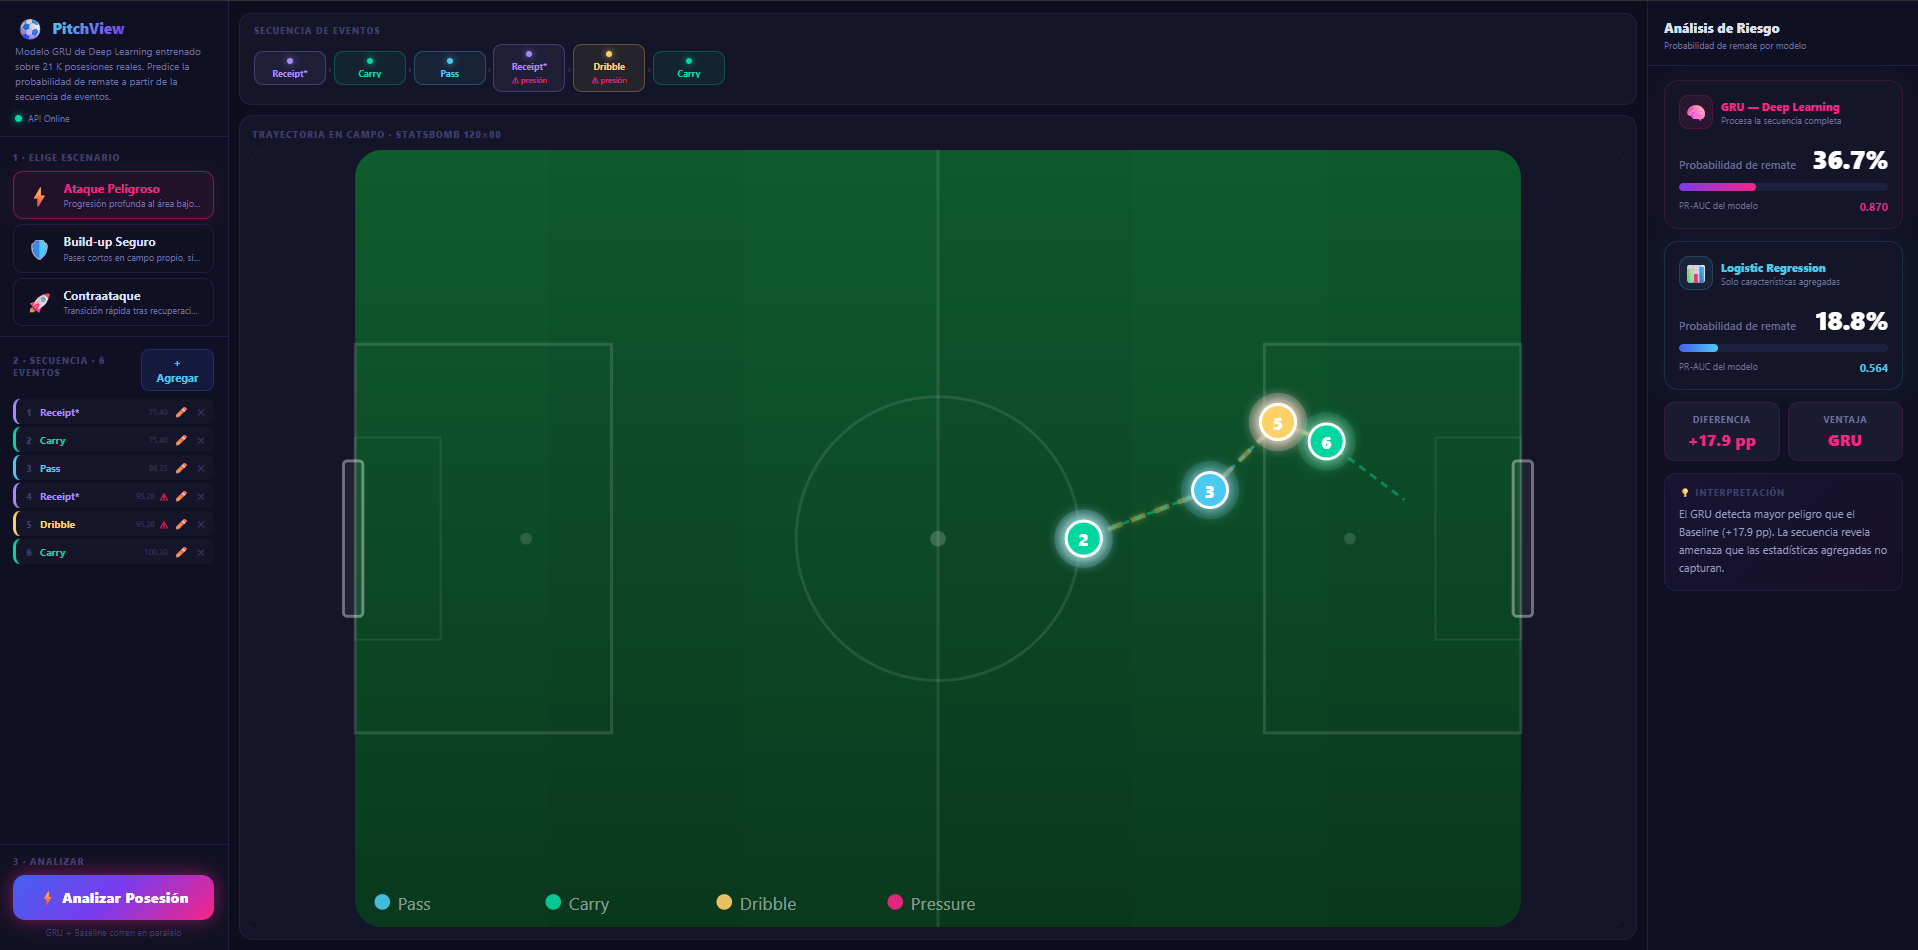
\includegraphics[width=\linewidth]{figures/app_ataque.png}
    \caption{PitchView — escenario \textit{Ataque Peligroso}: trayectoria de la posesión en campo, análisis comparativo GRU vs.\ Baseline con barras de probabilidad animadas e interpretación automática.}
    \label{fig:app_ataque}
\end{figure}

\begin{figure}[H]
    \centering
    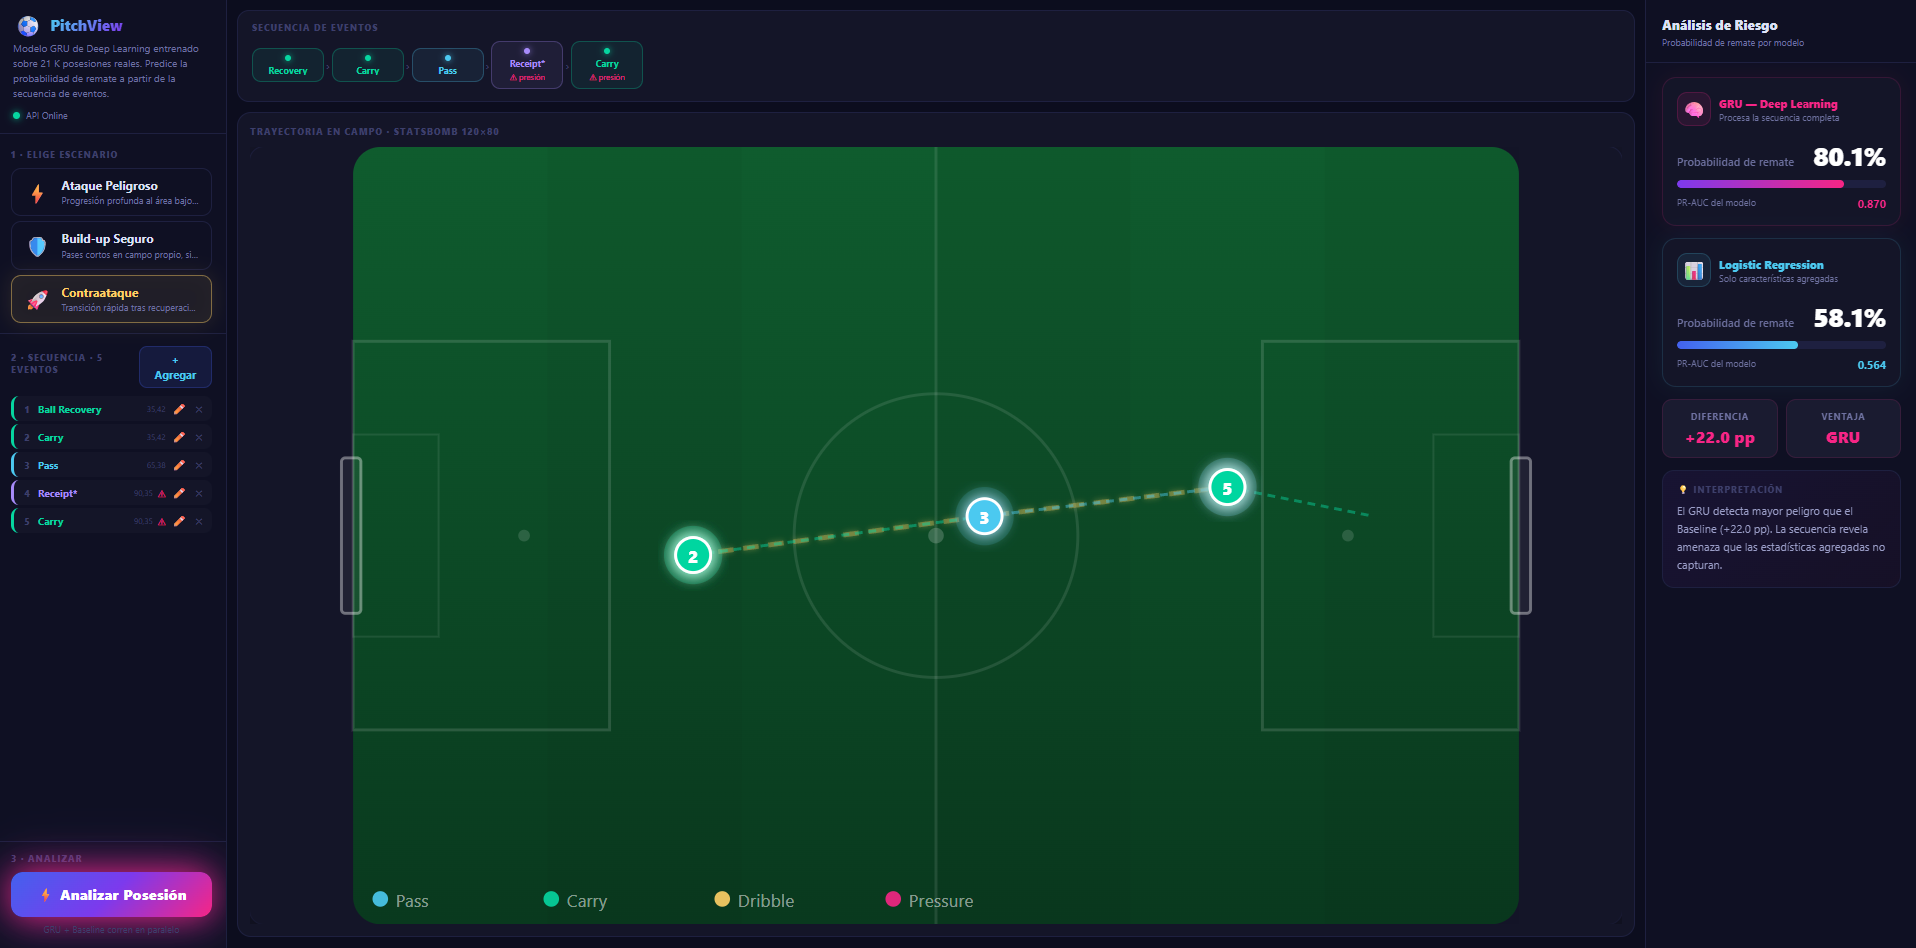
\includegraphics[width=\linewidth]{figures/app_contra.png}
    \caption{PitchView — escenario \textit{Contraataque}: transición rápida desde campo propio. La secuencia de eventos se muestra sobre el campo SVG y en la tira horizontal superior.}
    \label{fig:app_contra}
\end{figure}

\begin{figure}[H]
    \centering
    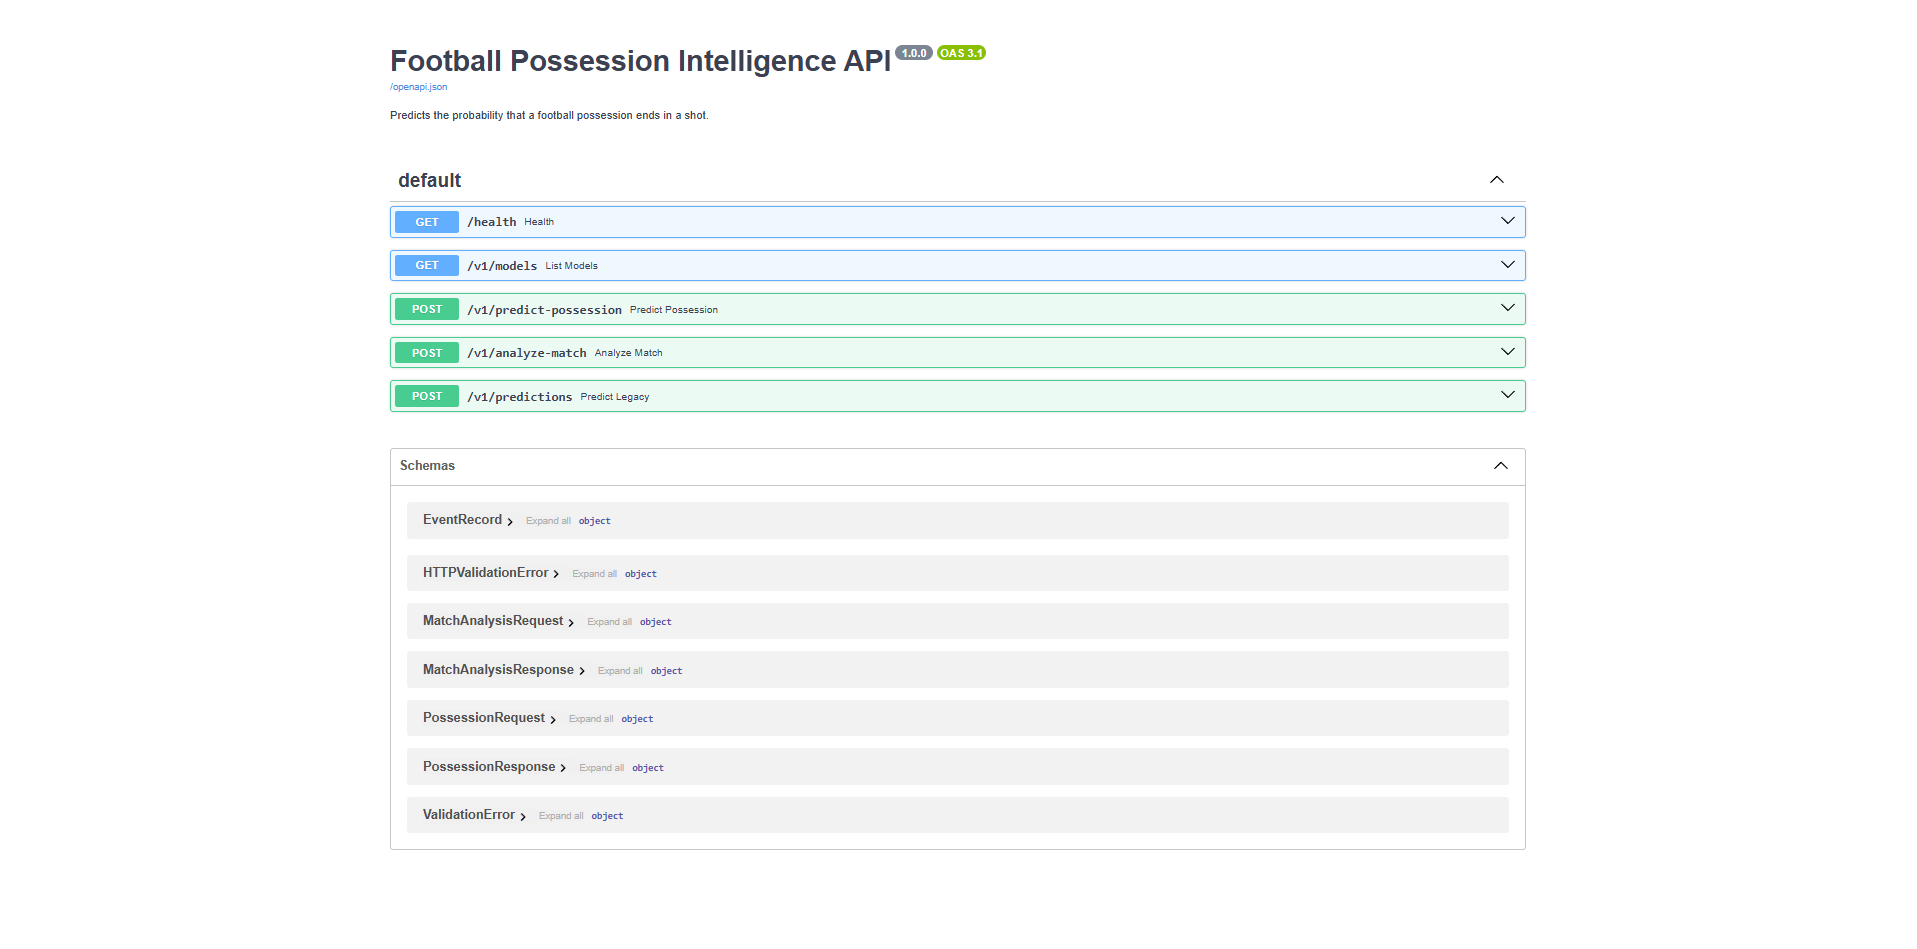
\includegraphics[width=\linewidth]{figures/app_docs.png}
    \caption{Documentación automática de la API en \texttt{/docs} (Swagger UI). Muestra los endpoints disponibles, el esquema JSON del request y la respuesta con \texttt{shot\_probability} y metadatos.}
    \label{fig:app_docs}
\end{figure}


%% ═══════════════════════════════════════════════════════════════
\section{Discusión}

\subsection{Interpretación de los resultados}

El modelo GRU supera ampliamente al baseline tabular en todas las métricas y ligas.
Esta brecha de $+30.7$~pp en PR-AUC no es trivial: demuestra que la \emph{secuencia}
de eventos contiene información predictiva que no está capturada por los agregados.
Aspectos como el orden de las acciones, la progresión incremental hacia la portería
o la acumulación de presión defensiva son patrones que el GRU puede capturar y el
baseline no.

Los resultados son estables entre validación y prueba (PR-AUC de $0.852$ y $0.870$
respectivamente), lo que sugiere buena generalización dentro del dominio de los
clubes europeos analizados.

\subsection{Limitaciones}

\begin{enumerate}[leftmargin=1.5em]
    \item \textbf{Representatividad del dataset:} 127 partidos de cuatro competencias
          es un dataset relativamente pequeño para deep learning. Modelos de producción
          como los de StatsBomb o Google DeepMind utilizan miles de partidos.
    \item \textbf{Vista post-hoc de la posesión:} El modelo ve la posesión completa
          (hasta su terminación), no el estado parcial en tiempo real. Para predicción
          en vivo se requeriría una evaluación adicional con secuencias truncadas.
    \item \textbf{Ausencia de contexto espacial 360°:} Los datos de \textit{freeze frame}
          (posición de todos los jugadores en el instante de cada evento) están disponibles
          en StatsBomb para estas competencias pero no fueron integrados en esta versión.
    \item \textbf{Calibración imperfecta:} El GRU muestra sobreconfianza moderada
          en el rango medio de probabilidades. Para aplicaciones donde la probabilidad
          calibrada es crítica, se recomienda post-calibración con Platt scaling.
    \item \textbf{Dominio acotado:} El modelo no fue evaluado en torneos internacionales
          ni competencias femeninas; su transferibilidad a esos dominios es desconocida.
\end{enumerate}

\subsection{Trabajo futuro}

\begin{itemize}[leftmargin=1.5em, noitemsep]
    \item Integrar datos de freeze frame (360°) para añadir contexto espacial.
    \item Explorar una formulación en tiempo real (predicción tras cada evento).
    \item Ampliar el dataset a más temporadas y ligas.
    \item Añadir la tarea secundaria $P(\text{gol} \mid \text{posesión})$.
    \item Evaluar arquitecturas Transformer con datasets más grandes.
\end{itemize}


%% ═══════════════════════════════════════════════════════════════
\section{Conclusión}

Este proyecto demuestra que el modelado secuencial de posesiones de fútbol con
redes recurrentes produce predicciones significativamente superiores a los enfoques
basados en características agregadas.

El modelo GRU desarrollado alcanza un \metric{PR-AUC de 0.870 en el conjunto de prueba}
con 21{,}080 posesiones extraídas de 127 partidos europeos, superando en $+30.7$~pp
al baseline tabular. La pipeline completa — desde la descarga de datos hasta la API
de inferencia — es reproducible y está documentada.

El sistema está listo para ser demostrado como aplicación funcional: la API FastAPI
acepta secuencias de eventos y retorna probabilidades de disparo en tiempo real,
mientras que el frontend React proporciona una interfaz visual para análisis táctico.

Desde la perspectiva del aprendizaje profundo, el proyecto valida la elección de
GRU sobre Transformer para este tamaño de dataset, e ilustra la importancia de un
diseño experimental riguroso (split sin fuga, exclusión de señales triviales,
métricas apropiadas para clases desbalanceadas).


%% ═══════════════════════════════════════════════════════════════
\appendix

\section{Glosario}
\label{app:glosario}

\begin{description}[leftmargin=2em, style=nextline]
    \item[Posesión] Secuencia continua de eventos realizados por el mismo equipo,
          identificada por el campo \code{possession} en los datos de StatsBomb.
    \item[GRU] \textit{Gated Recurrent Unit}. Variante simplificada de LSTM con dos
          puertas (actualización y reinicio) en lugar de tres.
    \item[PR-AUC] Área bajo la curva Precisión-Recall. Métrica robusta para datasets
          con desequilibrio de clases; un clasificador aleatorio obtiene PR-AUC $\approx$ tasa base.
    \item[ROC-AUC] Área bajo la curva Receiver Operating Characteristic. Mide la
          capacidad discriminativa del modelo independientemente del umbral de decisión.
    \item[BCE] \textit{Binary Cross-Entropy}. Función de pérdida estándar para
          clasificación binaria: $\mathcal{L} = -[y\log\hat{y} + (1-y)\log(1-\hat{y})]$.
    \item[Pack padded sequence] Técnica de PyTorch que comprime las secuencias
          eliminando el padding durante el procesamiento RNN para mayor eficiencia.
    \item[Freeze frame] Dato de StatsBomb 360° que captura la posición de todos
          los jugadores visibles en el campo en el momento de un evento.
    \item[xG] \textit{Expected Goals}. Probabilidad de que un disparo específico
          resulte en gol, basada en características del disparo. Distinto de
          $P(\text{disparo}\mid\text{posesión})$ que es lo que este proyecto predice.
\end{description}

\end{document}
